% !TeX spellcheck = hu_HU
% !TeX encoding = UTF-8
% !TeX program = xelatex
\documentclass[11pt,a4paper,oneside]{report}             % Single-side
%\documentclass[11pt,a4paper,twoside,openright]{report}  % Duplex

% thanks to http://tex.stackexchange.com/a/47579/71109
\usepackage{ifxetex}
\usepackage{ifluatex}
\newif\ifxetexorluatex % a new conditional starts as false
\ifnum 0\ifxetex 1\fi\ifluatex 1\fi>0
   \xetexorluatextrue
\fi

\ifxetexorluatex
  \usepackage{fontspec}
\else
  \usepackage[T1]{fontenc}
  \usepackage[utf8]{inputenc}
  \usepackage[lighttt]{lmodern}
\fi

\usepackage[english,magyar]{babel} % Alapértelmezés szerint utoljára definiált nyelv lesz aktív, de később külön beállítjuk az aktív nyelvet.

%\usepackage{cmap}
\usepackage{amsfonts,amsmath,amssymb} % Mathematical symbols.
%\usepackage[ruled,boxed,resetcount,linesnumbered]{algorithm2e} % For pseudocodes. % beware: this is not compatible with LuaLaTeX, see http://tex.stackexchange.com/questions/34814/lualatex-and-algorithm2e
\usepackage{booktabs} % For publication quality tables for LaTeX
\usepackage{graphicx}

%\usepackage{fancyhdr}
%\usepackage{lastpage}

\usepackage{anysize}
%\usepackage{sectsty}
\usepackage{setspace} % For setting line spacing

\usepackage[unicode]{hyperref} % For hyperlinks in the generated document.
\usepackage{xcolor}
\usepackage{listings} % For source code snippets.

\usepackage[amsmath,thmmarks]{ntheorem} % Theorem-like environments.

\usepackage[hang]{caption}

\singlespacing

\newcommand{\selecthungarian}{
	\selectlanguage{magyar}
	\setlength{\parindent}{2em}
	\setlength{\parskip}{0em}
	\frenchspacing
}

\newcommand{\selectenglish}{
	\selectlanguage{english}
	\setlength{\parindent}{0em}
	\setlength{\parskip}{0.5em}
	\nonfrenchspacing
	\renewcommand{\figureautorefname}{Figure}
	\renewcommand{\tableautorefname}{Table}
	\renewcommand{\partautorefname}{Part}
	\renewcommand{\chapterautorefname}{Chapter}
	\renewcommand{\sectionautorefname}{Section}
	\renewcommand{\subsectionautorefname}{Section}
	\renewcommand{\subsubsectionautorefname}{Section}
}

\usepackage[numbers]{natbib}
\usepackage{xspace}


\newcommand{\vikszerzoVezeteknev}{Nánási}
\newcommand{\vikszerzoKeresztnev}{Dániel}

\newcommand{\vikkonzulensAMegszolitas}{Dr. }
\newcommand{\vikkonzulensAVezeteknev}{Simon}
\newcommand{\vikkonzulensAKeresztnev}{Csaba}

\newcommand{\vikkonzulensBMegszolitas}{}
\newcommand{\vikkonzulensBVezeteknev}{}
\newcommand{\vikkonzulensBKeresztnev}{}

\newcommand{\vikkonzulensCMegszolitas}{}
\newcommand{\vikkonzulensCVezeteknev}{}
\newcommand{\vikkonzulensCKeresztnev}{}

\newcommand{\vikcim}{Felhő alapú drónvezérlés} % Cím
\newcommand{\viktanszek}{\bmetmit} % Tanszék
\newcommand{\vikdoktipus}{\msc} % Dokumentum típusa (\bsc vagy \msc)
\newcommand{\vikmunkatipusat}{szakdolgozatot} % a "hallgató nyilatkozat" részhez: szakdolgozatot vagy diplomatervet

%--------------------------------------------------------------------------------------
% TDK-specifikus változók
%--------------------------------------------------------------------------------------
\newcommand{\tdkszerzoB}{Második Szerző} % Második szerző neve; hagyd üresen, ha egyedül írtad a TDK-t.
\newcommand{\tdkev}{2014} % A dolgozat írásának éve (pl. "2014") (Ez OTDK-nál eltérhet az aktuális évtől.)

% További adatok az OTDK címlaphoz (BME-s TDK-hoz nem kell kitölteni)
\newcommand{\tdkevfolyamA}{IV} % Első szerző évfolyama, római számmal (pl. IV).
\newcommand{\tdkevfolyamB}{III} % Második szerző évfolyama, római számmal (pl. III).
\newcommand{\tdkkonzulensbeosztasA}{egyetemi tanár} % Első konzulens beosztása (pl. egyetemi docens)
\newcommand{\tdkkonzulensbeosztasB}{doktorandusz} % Második konzulens beosztása (pl. egyetemi docens)

\newcommand{\szerzoMeta}{\vikszerzoVezeteknev{} \vikszerzoKeresztnev} % egy szerző esetén
%\newcommand{\szerzoMeta}{\vikszerzoVezeteknev{} \vikszerzoKeresztnev, \tdkszerzoB} % két szerző esetén

% Beállítások magyar nyelvű dolgozathoz
%%--------------------------------------------------------------------------------------
% Elnevezések
%--------------------------------------------------------------------------------------
\newcommand{\bme}{Budapesti Műszaki és Gazdaságtudományi Egyetem}
\newcommand{\vik}{Villamosmérnöki és Informatikai Kar}

\newcommand{\bmemit}{Méréstechnika és Információs Rendszerek Tanszék}
\newcommand{\bmetmit}{Távközlési és Médiainformatikai Tanszék}

\newcommand{\keszitette}{Készítette}
\newcommand{\konzulens}{Konzulens}

\newcommand{\bsc}{Szakdolgozat}
\newcommand{\msc}{Diplomaterv}
\newcommand{\tdk}{TDK dolgozat}
\newcommand{\bsconlab}{BSc Önálló laboratórium}
\newcommand{\msconlabi}{MSc Önálló laboratórium 1.}
\newcommand{\msconlabii}{MSc Önálló laboratórium 2.}

\newcommand{\pelda}{Példa}
\newcommand{\definicio}{Definíció}
\newcommand{\tetel}{Tétel}

\newcommand{\bevezetes}{Bevezetés}
\newcommand{\koszonetnyilvanitas}{Köszönetnyilvánítás}
\newcommand{\fuggelek}{Függelék}

% Opcionálisan átnevezhető címek
%\addto\captionsmagyar{%
%\renewcommand{\listfigurename}{Saját ábrajegyzék cím}
%\renewcommand{\listtablename}{Saját táblázatjegyzék cím}
%\renewcommand{\bibname}{Saját irodalomjegyzék név}
%}


\newcommand{\szerzo}{\vikszerzoVezeteknev{} \vikszerzoKeresztnev}
\newcommand{\vikkonzulensA}{\vikkonzulensAMegszolitas\vikkonzulensAVezeteknev{} \vikkonzulensAKeresztnev}
\newcommand{\vikkonzulensB}{\vikkonzulensBMegszolitas\vikkonzulensBVezeteknev{} \vikkonzulensBKeresztnev}
\newcommand{\vikkonzulensC}{\vikkonzulensCMegszolitas\vikkonzulensCVezeteknev{} \vikkonzulensCKeresztnev}

\newcommand{\selectthesislanguage}{\selecthungarian}

\bibliographystyle{huplain}

\def\lstlistingname{lista}

\newcommand{\appendixnumber}{6}  % a fofejezet-szamlalo az angol ABC 6. betuje (F) lesz

% Settings for English documents
%--------------------------------------------------------------------------------------
% Elnevezések
%--------------------------------------------------------------------------------------
\newcommand{\bme}{Budapesti Műszaki és Gazdaságtudományi Egyetem}
\newcommand{\vik}{Villamosmérnöki és Informatikai Kar}

\newcommand{\bmemit}{Méréstechnika és Információs Rendszerek Tanszék}
\newcommand{\bmetmit}{Távközlési és Médiainformatikai Tanszék}

\newcommand{\keszitette}{Készítette}
\newcommand{\konzulens}{Konzulens}

\newcommand{\bsc}{Szakdolgozat}
\newcommand{\msc}{Diplomaterv}
\newcommand{\tdk}{TDK dolgozat}
\newcommand{\bsconlab}{BSc Önálló laboratórium}
\newcommand{\msconlabi}{MSc Önálló laboratórium 1.}
\newcommand{\msconlabii}{MSc Önálló laboratórium 2.}

\newcommand{\pelda}{Példa}
\newcommand{\definicio}{Definíció}
\newcommand{\tetel}{Tétel}

\newcommand{\bevezetes}{Bevezetés}
\newcommand{\koszonetnyilvanitas}{Köszönetnyilvánítás}
\newcommand{\fuggelek}{Függelék}

% Opcionálisan átnevezhető címek
%\addto\captionsmagyar{%
%\renewcommand{\listfigurename}{Saját ábrajegyzék cím}
%\renewcommand{\listtablename}{Saját táblázatjegyzék cím}
%\renewcommand{\bibname}{Saját irodalomjegyzék név}
%}


\newcommand{\szerzo}{\vikszerzoVezeteknev{} \vikszerzoKeresztnev}
\newcommand{\vikkonzulensA}{\vikkonzulensAMegszolitas\vikkonzulensAVezeteknev{} \vikkonzulensAKeresztnev}
\newcommand{\vikkonzulensB}{\vikkonzulensBMegszolitas\vikkonzulensBVezeteknev{} \vikkonzulensBKeresztnev}
\newcommand{\vikkonzulensC}{\vikkonzulensCMegszolitas\vikkonzulensCVezeteknev{} \vikkonzulensCKeresztnev}

\newcommand{\selectthesislanguage}{\selecthungarian}

\bibliographystyle{huplain}

\def\lstlistingname{lista}

\newcommand{\appendixnumber}{6}  % a fofejezet-szamlalo az angol ABC 6. betuje (F) lesz

%--------------------------------------------------------------------------------------
% Page layout setup
%--------------------------------------------------------------------------------------
% we need to redefine the pagestyle plain
% another possibility is to use the body of this command without \fancypagestyle
% and use \pagestyle{fancy} but in that case the special pages
% (like the ToC, the References, and the Chapter pages)remain in plane style

\pagestyle{plain}
\marginsize{35mm}{25mm}{15mm}{15mm}

\setcounter{tocdepth}{3}
%\sectionfont{\large\upshape\bfseries}
\setcounter{secnumdepth}{3}

\sloppy % Margón túllógó sorok tiltása.
\widowpenalty=10000 \clubpenalty=10000 %A fattyú- és árvasorok elkerülése
\def\hyph{-\penalty0\hskip0pt\relax} % Kötőjeles szavak elválasztásának engedélyezése


%--------------------------------------------------------------------------------------
% Setup hyperref package
%--------------------------------------------------------------------------------------
\hypersetup{
    % bookmarks=true,            % show bookmarks bar?
    unicode=true,              % non-Latin characters in Acrobat's bookmarks
    pdftitle={\vikcim},        % title
    pdfauthor={\szerzoMeta},    % author
    pdfsubject={\vikdoktipus}, % subject of the document
    pdfcreator={\szerzoMeta},   % creator of the document
    pdfproducer={},    % producer of the document
    pdfkeywords={},    % list of keywords (separate then by comma)
    pdfnewwindow=true,         % links in new window
    colorlinks=true,           % false: boxed links; true: colored links
    linkcolor=black,           % color of internal links
    citecolor=black,           % color of links to bibliography
    filecolor=black,           % color of file links
    urlcolor=black             % color of external links
}


%--------------------------------------------------------------------------------------
% Set up listings
%--------------------------------------------------------------------------------------
\definecolor{lightgray}{rgb}{0.95,0.95,0.95}
\lstset{
	basicstyle=\scriptsize\ttfamily, % print whole listing small
	keywordstyle=\color{black}\bfseries, % bold black keywords
	identifierstyle=, % nothing happens
	% default behavior: comments in italic, to change use
	% commentstyle=\color{green}, % for e.g. green comments
	stringstyle=\scriptsize,
	showstringspaces=false, % no special string spaces
	aboveskip=3pt,
	belowskip=3pt,
	backgroundcolor=\color{lightgray},
	columns=flexible,
	keepspaces=true,
	escapeinside={(*@}{@*)},
	captionpos=b,
	breaklines=true,
	frame=single,
	float=!ht,
	tabsize=2,
	literate=*
		{á}{{\'a}}1	{é}{{\'e}}1	{í}{{\'i}}1	{ó}{{\'o}}1	{ö}{{\"o}}1	{ő}{{\H{o}}}1	{ú}{{\'u}}1	{ü}{{\"u}}1	{ű}{{\H{u}}}1
		{Á}{{\'A}}1	{É}{{\'E}}1	{Í}{{\'I}}1	{Ó}{{\'O}}1	{Ö}{{\"O}}1	{Ő}{{\H{O}}}1	{Ú}{{\'U}}1	{Ü}{{\"U}}1	{Ű}{{\H{U}}}1
}


%--------------------------------------------------------------------------------------
% Set up theorem-like environments
%--------------------------------------------------------------------------------------
% Using ntheorem package -- see http://www.math.washington.edu/tex-archive/macros/latex/contrib/ntheorem/ntheorem.pdf

\theoremstyle{plain}
\theoremseparator{.}
\newtheorem{example}{\pelda}

\theoremseparator{.}
%\theoremprework{\bigskip\hrule\medskip}
%\theorempostwork{\hrule\bigskip}
\theorembodyfont{\upshape}
\theoremsymbol{{\large \ensuremath{\centerdot}}}
\newtheorem{definition}{\definicio}

\theoremseparator{.}
%\theoremprework{\bigskip\hrule\medskip}
%\theorempostwork{\hrule\bigskip}
\newtheorem{theorem}{\tetel}


%--------------------------------------------------------------------------------------
% Some new commands and declarations
%--------------------------------------------------------------------------------------
\newcommand{\code}[1]{{\upshape\ttfamily\scriptsize\indent #1}}
\newcommand{\doi}[1]{DOI: \href{http://dx.doi.org/\detokenize{#1}}{\raggedright{\texttt{\detokenize{#1}}}}} % A hivatkozások közt így könnyebb DOI-t megadni.

\DeclareMathOperator*{\argmax}{arg\,max}
%\DeclareMathOperator*[1]{\floor}{arg\,max}
\DeclareMathOperator{\sign}{sgn}
\DeclareMathOperator{\rot}{rot}


%--------------------------------------------------------------------------------------
% Setup captions
%--------------------------------------------------------------------------------------
\captionsetup[figure]{
	width=.75\textwidth,
	aboveskip=10pt}

\renewcommand{\captionlabelfont}{\bf}
%\renewcommand{\captionfont}{\footnotesize\it}

%--------------------------------------------------------------------------------------
% Hyphenation exceptions
%--------------------------------------------------------------------------------------
\hyphenation{Shakes-peare Mar-seilles ár-víz-tű-rő tü-kör-fú-ró-gép}


\author{\vikszerzo}
\title{\viktitle}

%--------------------------------------------------------------------------------------
% Table of contents and the main text
%--------------------------------------------------------------------------------------
\begin{document}

\pagenumbering{gobble}
%~~~~~~~~~~~~~~~~~~~~~~~~~~~~~~~~~~~~~~~~~~~~~~~~~~~~~~~~~~~~~~~~~~~~~~~~~~~~~~~~~~~~~~
%\selecthungarian
%--------------------------------------------------------------------------------------
% Rovid formai es tartalmi tajekoztato
%--------------------------------------------------------------------------------------

\footnotesize
\begin{center}
\large
\textbf{\Large Általános információk, a diplomaterv szerkezete}\\
\end{center}

A diplomaterv szerkezete a BME Villamosmérnöki és Informatikai Karán:
\begin{enumerate}
\item	Diplomaterv feladatkiírás
\item	Címoldal
\item	Tartalomjegyzék
\item	A diplomatervező nyilatkozata az önálló munkáról és az elektronikus adatok kezeléséről
\item	Tartalmi összefoglaló magyarul és angolul
\item	Bevezetés: a feladat értelmezése, a tervezés célja, a feladat indokoltsága, a diplomaterv felépítésének rövid összefoglalása
\item	A feladatkiírás pontosítása és részletes elemzése
\item	Előzmények (irodalomkutatás, hasonló alkotások), az ezekből levonható következtetések
\item	A tervezés részletes leírása, a döntési lehetőségek értékelése és a választott megoldások indoklása
\item	A megtervezett műszaki alkotás értékelése, kritikai elemzése, továbbfejlesztési lehetőségek
\item	Esetleges köszönetnyilvánítások
\item	Részletes és pontos irodalomjegyzék
\item	Függelék(ek)
\end{enumerate}

Felhasználható a következő oldaltól kezdődő \LaTeX diplomatervsablon dokumentum tartalma. 

A diplomaterv szabványos méretű A4-es lapokra kerüljön. Az oldalak tükörmargóval készüljenek (mindenhol 2,5~cm, baloldalon 1~cm-es kötéssel). Az alapértelmezett betűkészlet a 12 pontos Times New Roman, másfeles sorközzel, de ettől kismértékben el lehet térni, ill. más betűtípus használata is megengedett.

Minden oldalon -- az első négy szerkezeti elem kivételével -- szerepelnie kell az oldalszámnak.

A fejezeteket decimális beosztással kell ellátni. Az ábrákat a megfelelő helyre be kell illeszteni, fejezetenként decimális számmal és kifejező címmel kell ellátni. A fejezeteket decimális aláosztással számozzuk, maximálisan 3 aláosztás mélységben (pl. 2.3.4.1.). Az ábrákat, táblázatokat és képleteket célszerű fejezetenként külön számozni (pl. 2.4. ábra, 4.2. táblázat vagy képletnél (3.2)). A fejezetcímeket igazítsuk balra, a normál szövegnél viszont használjunk sorkiegyenlítést. Az ábrákat, táblázatokat és a hozzájuk tartozó címet igazítsuk középre. A cím a jelölt rész alatt helyezkedjen el.

A képeket lehetőleg rajzoló programmal készítsék el, az egyenleteket egyenlet-szerkesztő segítségével írják le (A \LaTeX~ehhez kézenfekvő megoldásokat nyújt).

Az irodalomjegyzék szövegközi hivatkozása történhet sorszámozva (ez a preferált megoldás) vagy a Harvard-rendszerben (a szerző és az évszám megadásával). A teljes lista névsor szerinti sorrendben a szöveg végén szerepeljen (sorszámozott irodalmi hivatkozások esetén hivatkozási sorrendben). A szakirodalmi források címeit azonban mindig az eredeti nyelven kell megadni, esetleg zárójelben a fordítással. A listában szereplő valamennyi publikációra hivatkozni kell a szövegben (a \LaTeX-sablon a Bib\TeX~segítségével mindezt automatikusan kezeli). Minden publikáció a szerzők után a következő adatok szerepelnek: folyóirat cikkeknél a pontos cím, a folyóirat címe, évfolyam, szám, oldalszám tól-ig. A folyóiratok címét csak akkor rövidítsük, ha azok nagyon közismertek vagy nagyon hosszúak. Internetes hivatkozások megadásakor fontos, hogy az elérési út előtt megadjuk az oldal tulajdonosát és tartalmát (mivel a link egy idő után akár elérhetetlenné is válhat), valamint az elérés időpontját.

\vspace{5mm}
Fontos:
\begin{itemize}
	\item A szakdolgozatkészítő / diplomatervező nyilatkozata (a jelen sablonban szereplő szövegtartalommal) kötelező előírás, Karunkon ennek hiányában a szakdolgozat/diplomaterv nem bírálható és nem védhető!
	\item Mind a dolgozat, mind a melléklet maximálisan 15~MB méretű lehet!
\end{itemize}

\vspace{5mm}
\begin{center}
Jó munkát, sikeres szakdolgozatkészítést, ill. diplomatervezést kívánunk!
\end{center}

\normalsize
\selectthesislanguage

%%--------------------------------------------------------------------------------------
% Feladatkiiras (a tanszeken atveheto, kinyomtatott valtozat)
%--------------------------------------------------------------------------------------
\clearpage
\begin{center}
\large
\textbf{FELADATKIÍRÁS}\\
\end{center}

A feladatkiírást a tanszéki adminisztrációban lehet átvenni, és a leadott munkába eredeti, tanszéki pecséttel ellátott és a tanszékvezető által aláírt lapot kell belefűzni (ezen oldal \emph{helyett}, ez az oldal csak útmutatás). Az elektronikusan feltöltött dolgozatban már nem kell beleszerkeszteni ezt a feladatkiírást.


\selectthesislanguage

%~~~~~~~~~~~~~~~~~~~~~~~~~~~~~~~~~~~~~~~~~~~~~~~~~~~~~~~~~~~~~~~~~~~~~~~~~~~~~~~~~~~~~~
%\hypersetup{pageanchor=false}
%--------------------------------------------------------------------------------------
%	The title page
%--------------------------------------------------------------------------------------
\begin{titlepage}
\begin{center}

\includegraphics[width=60mm,keepaspectratio]{figures/bme_logo.pdf}\\
\vspace{0.3cm}
\textbf{\bme}\\
\textmd{\vik}\\
\textmd{\viktanszek}\\[5cm]

\vspace{0.4cm}
{\huge \bfseries \vikcim}\\[0.8cm]
\vspace{0.5cm}
\textsc{\Large \vikdoktipus}\\[4cm]

{
	\renewcommand{\arraystretch}{0.85}
	\begin{tabular}{cc}
	 \makebox[7cm]{\emph{\keszitette}} & \makebox[7cm]{\emph{\konzulens}} \\ \noalign{\smallskip}
	 \makebox[7cm]{\szerzo} & \makebox[7cm]{\vikkonzulensA} \\
	  & \makebox[7cm]{\vikkonzulensB} \\
	  & \makebox[7cm]{\vikkonzulensC} \\
	\end{tabular}
}

\vfill
{\large 2020. December}
\end{center}
\end{titlepage}
\hypersetup{pageanchor=false}

		   % Szakdolgozat/Diplomaterv címlap

% Table of Contents
%~~~~~~~~~~~~~~~~~~~~~~~~~~~~~~~~~~~~~~~~~~~~~~~~~~~~~~~~~~~~~~~~~~~~~~~~~~~~~~~~~~~~~~
\tableofcontents\vfill


% Declaration and Abstract
%~~~~~~~~~~~~~~~~~~~~~~~~~~~~~~~~~~~~~~~~~~~~~~~~~~~~~~~~~~~~~~~~~~~~~~~~~~~~~~~~~~~~~~
%\selectlanguage{magyar}
\pagenumbering{gobble}
%--------------------------------------------------------------------------------------
% Nyilatkozat
%--------------------------------------------------------------------------------------
\begin{center}
\large
\textbf{HALLGATÓI NYILATKOZAT}\\
\end{center}

Alulírott \emph{\vikszerzoVezeteknev{} \vikszerzoKeresztnev}, szigorló hallgató kijelentem, hogy ezt a \vikmunkatipusat{} meg nem engedett segítség nélkül, saját magam készítettem, csak a megadott forrásokat (szakirodalom, eszközök stb.) használtam fel. Minden olyan részt, melyet szó szerint, vagy azonos értelemben, de átfogalmazva más forrásból átvettem, egyértelműen, a forrás megadásával megjelöltem.

Hozzájárulok, hogy a jelen munkám alapadatait (szerző(k), cím, angol és magyar nyelvű tartalmi kivonat, készítés éve, konzulens(ek) neve) a BME VIK nyilvánosan hozzáférhető elektronikus formában, a munka teljes szövegét pedig az egyetem belső hálózatán keresztül (vagy autentikált felhasználók számára) közzétegye. Kijelentem, hogy a benyújtott munka és annak elektronikus verziója megegyezik. Dékáni engedéllyel titkosított diplomatervek esetén a dolgozat szövege csak 3 év eltelte után válik hozzáférhetővé.

\begin{flushleft}
\vspace*{1cm}
Budapest, \today
\end{flushleft}

\begin{flushright}
 \vspace*{1cm}
 \makebox[7cm]{\rule{6cm}{.4pt}}\\
 \makebox[7cm]{\emph{\vikszerzoVezeteknev{} \vikszerzoKeresztnev}}\\
 \makebox[7cm]{hallgató}
\end{flushright}
\thispagestyle{empty}

\vfill
\clearpage
\thispagestyle{empty} % an empty page

\selectthesislanguage
 %TODO Hallgatói nyilatkozat -- TDK és OTDK esetén törlendő!
%%\pagenumbering{roman}
%\setcounter{page}{1}

\selecthungarian

%----------------------------------------------------------------------------
% Abstract in Hungarian
%----------------------------------------------------------------------------
\chapter*{Kivonat}\addcontentsline{toc}{chapter}{Kivonat}

A diplomaterv a mai felhőrendszerekről és azokban robot irányítási megoldásaiban mélyed el.
Megmutatja a mai rendszerek felhőrendszerek szolgáltatás alapú technológiáit és bevezeti az olvasót a konténeralapú szolgáltatásmenedzsmentbe. Leírást ad a felhasználói igényekről és a felhőrendszereknek a jövőbeli fejlesztési lehetőségeiről. Áttekintést ad a közösségi fejlesztések által nyújtott nagy méretű erőforrás menedzsment megoldásoknak a mikéntjére, azok hibájára és bemutatja tesztelésüket. A dolgozat ismerteti és feldolgozza a mai robotirányítási megoldásokat, kifejezett prioritást tekintve a drón irányításnak, azoknak ipari felhasználásáról és megvalósíthatóságáról. Betekintést ad miként valósítható meg egy 5G kommunikációra alapuló robotirányításra tervezett felhőrendszer. Megmutat egy nagyobb számú robotot központi konténer alapú vezérlő és jelfeldolgozó rendszer megvalósítást. Továbbá kifejti ezeknek a tervezési és implementációs lépéseit és a távvezérlési funkciók dinamikus elhelyezését megvalósító módszert. Szimulációt mutat nagyszámú robotvezérlés és annak kamerajelének feldolgozására a kialakított rendszerben. Ennek tükrében összeveti a drónvezérlés QoS (Quality of Service) igényeinek feltételeit és a megvalósított rendszer funkcióinak ezen feltételrendszerre szabott tervezési megoldást ad a felhő rendszeren belül!
Összefoglalja az elvégzett munkát, a szimuláció eredményeit és a QoS feltételrendszert a kialakított tesztrendszerben.


\vfill
\selectenglish


%----------------------------------------------------------------------------
% Abstract in English
%----------------------------------------------------------------------------
\chapter*{Abstract}\addcontentsline{toc}{chapter}{Abstract}

The thesis delves into today’s cloud systems and the control solutions of individual robots.
It demonstrates today’s systems with cloud-based service technologies and introduces readers to container-based service management. Provides a description of user needs and cloud systems. Overview and a community development of large-scale resource management solutions is a way of failing and presenting their testing. The thesis describes and processes robot control solutions with explicit priority for drone guidelines, industrial use, and applicability. Provides insight into how to implement a cloud system designed for robotic control based on a 5G communication system. It focuses for larger number of robots in the operation of a central container-based control and signal processing system. In addition, it shows the design and implementation steps as well as the dynamic placement of remote control functions in the system design methodology. It analyses results of simulations in a system created to process a large number of robot controls and their camera signals. In order to improve quality, in order to facilitate the use of QoS (Quality of Service) and to facilitate the operation of the established system, the conditionalities usually becomes available.
Summarize the work, simulation, development and QoS conditions of the test system.

\vfill
\selectthesislanguage

\newcounter{romanPage}
\setcounter{romanPage}{\value{page}}
\stepcounter{romanPage}    %TODO Összefoglaló -- TDK és OTDK esetén nem kötelező


% The main part of the thesis
%~~~~~~~~~~~~~~~~~~~~~~~~~~~~~~~~~~~~~~~~~~~~~~~~~~~~~~~~~~~~~~~~~~~~~~~~~~~~~~~~~~~~~~
\pagenumbering{arabic}
\chapter{Bevezetés}

Napjainkban a kisméretű repülő eszközöket, népszerű nevükön drónokat, sok feladatra használják. Jellemzően rádiós távvezérléssel, humán pilóta vezeti. Ugyanakkor elterjedőben van az automatizált feladatvezérlés is, de jelenleg főleg előre betáplált GPS koordináták sorozataként specikált útvonalat követnek. A mesterséges intelligencia technológia fejlődésével nagy reményt fűznek a feladatok programozott, adaptív logika alapú meghatározásával. Ebben az esetben a robotok vezérlését is meg kell oldani, a vezérlési logika által meghatározott koordináták alapján egy vezérlési központból küldik a parancsot a drónra. Mivel a vezérlési logika számításigényes, ezért ezt számítógép (adat) központokban futtatják és a vezérlési központ is a logika mellé van telepítve, valamint az adatközponotok tipikusan felhő rendszerként vannak megvalósítva. A munkám során egy ilyen felhőrendszerbe telepített vezérlési központ megvalósítási kérdéseivel foglalkoztam.

\section{Előzmények}

A dolgozatom témája felhő alapú drónvezérlés, amely több ágazatot, tématerületet ötvöz. Ugyanis a felhőtechnológiák, a robotvezérlés és az irányítástechnika spektrumot is lefedi a feladat, azonban én a felhőtechnológiák felől közelítem meg. A felhőalkalmazások ipara is egy ilyen terület, ahol bizonyos szolgáltatásokat minél szélesebb körben szeretnénk értékesíteni igény szerint, azonban valamilyen központi vezérlés működteti automatikusan az erőforráskiosztást, hozzáférést. A műhelyben végzett feladataim között felmerült a Kubernetes elosztott konténerkezelő rendszer, a Kubless serverless architektúra, felhő alapú beszédfelismerő rendszerek és az OpenStack virtuális gép menedzselő rendszer, amihez egy archiválási megoldást fejlesztettem szakdolgozatként. A felhő alapú drónirányítás téma a diplomatervem kezdetén került szóba, előtte nem foglalkoztam mélyebben robotirányítással és vezérléssel, így remélhetőleg ezekből a területekből is nagy tapasztalatot fogok szerezni a feladat befejeztén.

\section{A feladat célja}

\subsection{Feltételrendszer}
A feladat sokféleképpen általánosítható, hiszen egy felhőrendszerből igen sokféle ipari folyamatot lehet irányítani, csupán a megvalósítást kell kivitelezni. Egy drón irányítása sem különbözik, lehetne a cél robotkar vezérlése, gyártósor ütemezése, automatikus kötöttpályás közlekedési eszköz irányítása vagy akár önvezető autók feletti vezérlés.
 Azonban a témámban nem egy drón irányítását, hanem több, akár tíz-húszat is elérheti az a teszteset amire szeretnék megoldást adni. Egy ilyen rendszert irányító felhő architektrúban rugalmasabb és erőforrás takarékosabb üzemeltetést lehet elérni. A számításkapacitás optimalizáció nem minden amit ebben a helyzetben az ipar megkíván, hanem azokat a kommunikációs kapcsolatokat, amelyek szigorú minőségi elvárásoknak (Quality -of Service – QoS) kell megfelelniük, ezért bonyolultabb kezelni. A feladat feltérképezni a modern felhőrendszereket, amelyekkel meg lehet valósítani efféle iparban is használható vezérlési technikát QoS feltételek mellett. Tehát a projektnek három kritikus tervezési mérföldköve van. Ezeknek kapcsolata látszik a \ref{fig:merfold}. ábrán.
\begin{figure}
	\centering
	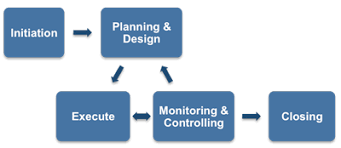
\includegraphics[width=10cm]{figures/plan_excecute_monitor.png}
	\caption{Kritikus mérföldkövek folyamata \cite{ProjecPlan}}
	\label{fig:merfold}
\end{figure}
\begin{enumerate}
	\item Kiválasztani a megfelelő felhőrendszert, amiben megvalósítható $R\in [1, 100]$ drón, vagy általánosan, valamilyen vezérelhető eszköz (robot) irányítása.
	\item Áttekinteni drónvezérlést támogató szoftver megoldásokat, kiválasztani egy olyan környezetet, mellyel távvezérlési funkciók megvalósíthatók. Megtervezni ebben a felhőrendszerben több drón irányítását és jelfeldolgozását, automatikusan és biztosítva, hogy hiba esetén visszaálljon a működő állapot.
	\item A meglévő rendszer analizálása, optimalizálása és egy QoS feltétel felállítása.
\end{enumerate}

\subsection{Vezérlési feladatok erőforrásigénye}
\noindent
Dolgozatom célja nem csak a drónirányítórendszer megvalósítása, hanem annak kapacitásának megbecslése is, akár  több tíz drón irányítására. Ezt a feltételt valamilyen $f_{QoS}(R,C)\in N^2$ függvény fogja megadni, melynek paraméterei $R$ a robotok száma és $C$ a számítási erőforrás. Ha számításról beszélünk, akkor a felhőszolgáltatások iparában kiválasztunk egy valamilyen optimális $c=$RAM[GB]/VCPU arányt mely az alkalmazásunkhoz megfelelő és annak $n\in N^+$, $C=c\cdot n$ egész számú többszöröse lesz a számítási kapacitás amire méretezünk. Vagyis valamilyen 2 dimenziós tervezési teret adunk meg a kívánt szolgáltatási minőség eléréséhez. Az ilyen jellegű feladatokban a szolgáltatás minősége általában a válaszidőt szokta jelenteni $n \cdot 10$-es nagyságrendben. Természetesen ez nem egy túl pontos modell, de egy mérnöki kapacitástervezés számára kellő kiindulási alapot adhat méretezni a felhőrendszert, esetleg skálázhatósági lehetőségeket is figyelembe véve.
Ezen kívül mivel nagyszámú eszközről beszélünk nem tekinthetünk el a közegátviteli technológiáról. Azt sejthetjük, hogy a mai elterjedt távközlő rendszerek nem alkalmasak akár száz fölötti felhasználóval, mondjuk robottal folyamatos kommunikációt tartani megfelelő QoS-el. Ezért megnézem, hogy a mai modern felhőrendszerekkel és az 5G között milyen kapcsolatot lehet alakítani és mik a feltételek egy ilyen rendszerben való üzemeltetéshez. \\

\subsection{Elvárások a rendszerrel szemben}
\noindent
A feladat megvalósított terméke pedig egy valamilyen automatizált felhőrendszerbe ültetett drónirányító központ melynek segítségével $N$ darab virtuális vagy fizikai drónt tudunk üzemeltetni, az előző bekezdésben taglalt QoS feltételek mellett. Fontos, hogy a drónirányító központban minden kommunikációt tudjunk kontrollálni és biztonságos állapotba helyezni a drónokat, hogyha tudjuk, hogy valamely biztosítandó alapfeltételnek nem tesz eleget pillanatnyilag a rendszerünk. Tehát amit meg kell valósítani a mérések mellett az nem más, mint egy felhőrendszerbe integrált szoftver, amely biztosítja 
\begin{itemize}
	\item előre definiált $N$ darab drón irányítását a felhasználónak, a felhőből kivezetett interfészen,
	\item minden drónra vonatkozó kamerakép és irányítási parancsok átviteli sebessége, előre definiált konstans alapján,
	\item a drón és felhő közötti kapcsolatot egy előre definiált minimum sávszélesség alapján,
	\item amennyiben az előző feltételeknek nem tesz eleget a rendszer, a biztonságos leállítását az összes drónnak.
\end{itemize}

\subsection{Sávszélesség}
\noindent
Ezen feltételek mellett felírhatunk pár egyszerű összefüggést egy vázlatos modellre, aminek blokkdiagramja a \ref{fig:dronecommunicationtocloud}. ábrán látható. Tudjuk, hogy lesz egy valamilyen még ki nem választott felhőrendszer, amely biztosan több node-ból fog állni, tehát több fizikai vagy virtuális gép fogja szolgáltatni a felhőrendszer platformját. A node-ok között feltételezzük, hogy nincs sávszélességi korlát. A felhőrendszer szolgáltat valamilyen interface-t amint elérhető az integrált szolgáltatás a drónok számára. Ezen modellen következik, hogy a hálózati interface és a tényleges integrált applikáció közötti sávszélességnek nagyobbnak kell lennie, mint a drón felé a sávszélesség összessége:
\begin{equation}
BWc \geq \sum_{i=1}^{n}{BWd_i}
\end{equation}

A drónok sávszélességére felírhatjuk azt a feltételt, amely kimondja, hogy bármely drón sávszélességének nagyobbnak kell lennie, mint a videófolyamhoz rendelt minimális sávszélességnek és az irányításhoz megszabott minimális irányíthatósági sávszélességnek.
\begin{equation}
\forall d \in D: BW_d \geq BWV_{min} + BWC_{min}
\end{equation}
Ahol $BWV_{min}$ a videó minimális sávszélessége, $BMC_{min}$ a kontrollerhez rendelt minimális sávszélesség, $BW_d$ az adott drón és a felhő közötti sávszélesség, $D$ pedig a drónok halmaza.

\begin{figure}
	\centering
	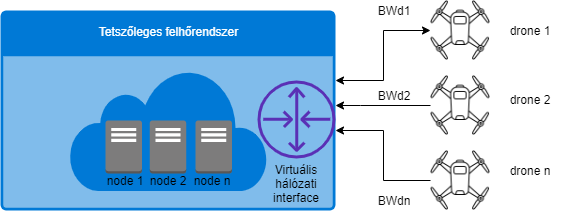
\includegraphics[width=\linewidth]{figures/drone_communication_to_cloud.png}
	\caption{A drónok és felhő kapcsolatának vázlatos modellje}
	\label{fig:dronecommunicationtocloud}
\end{figure}

\section{Feladat indokoltsága}
\subsection{Gyártóipar}
A nagyszámú eszközök irányítása számtalan szektorban elterjedt és alkalmazható. Akár beszélve a gyártó szektorról, ahol nagyon sok folyamatot robotok látnak el és legyen az bármilyen robot, az valószínűleg irányítható felhőből. Persze sokszor a gyártók egy drágább, de kapacitásban túlbiztosított lokális rendszerről irányítják a gyártórobotjaikat, mivel a felhős megoldások még annyira nem elterjedtek ebben a célfelhasználásban. Azonban egy ilyen megoldással rengeteg erőforrás megtakarítható.
A \ref{fig:industry40}. ábrán láthatóak az Ipar 4.0 főbb komponensei és könnyen meggyőződhetünk róla, hogy egy mai innovatív ipari környezetben inkább a felhő alapú megoldásokat választják a skálázhatóság és a biztonságuk miatt. Ebben az esetben felhőről általában számítási kapacitásról beszélünk, azonban később kitérünk a szolgáltatások kategóriáira.
\begin{figure}
	\centering
	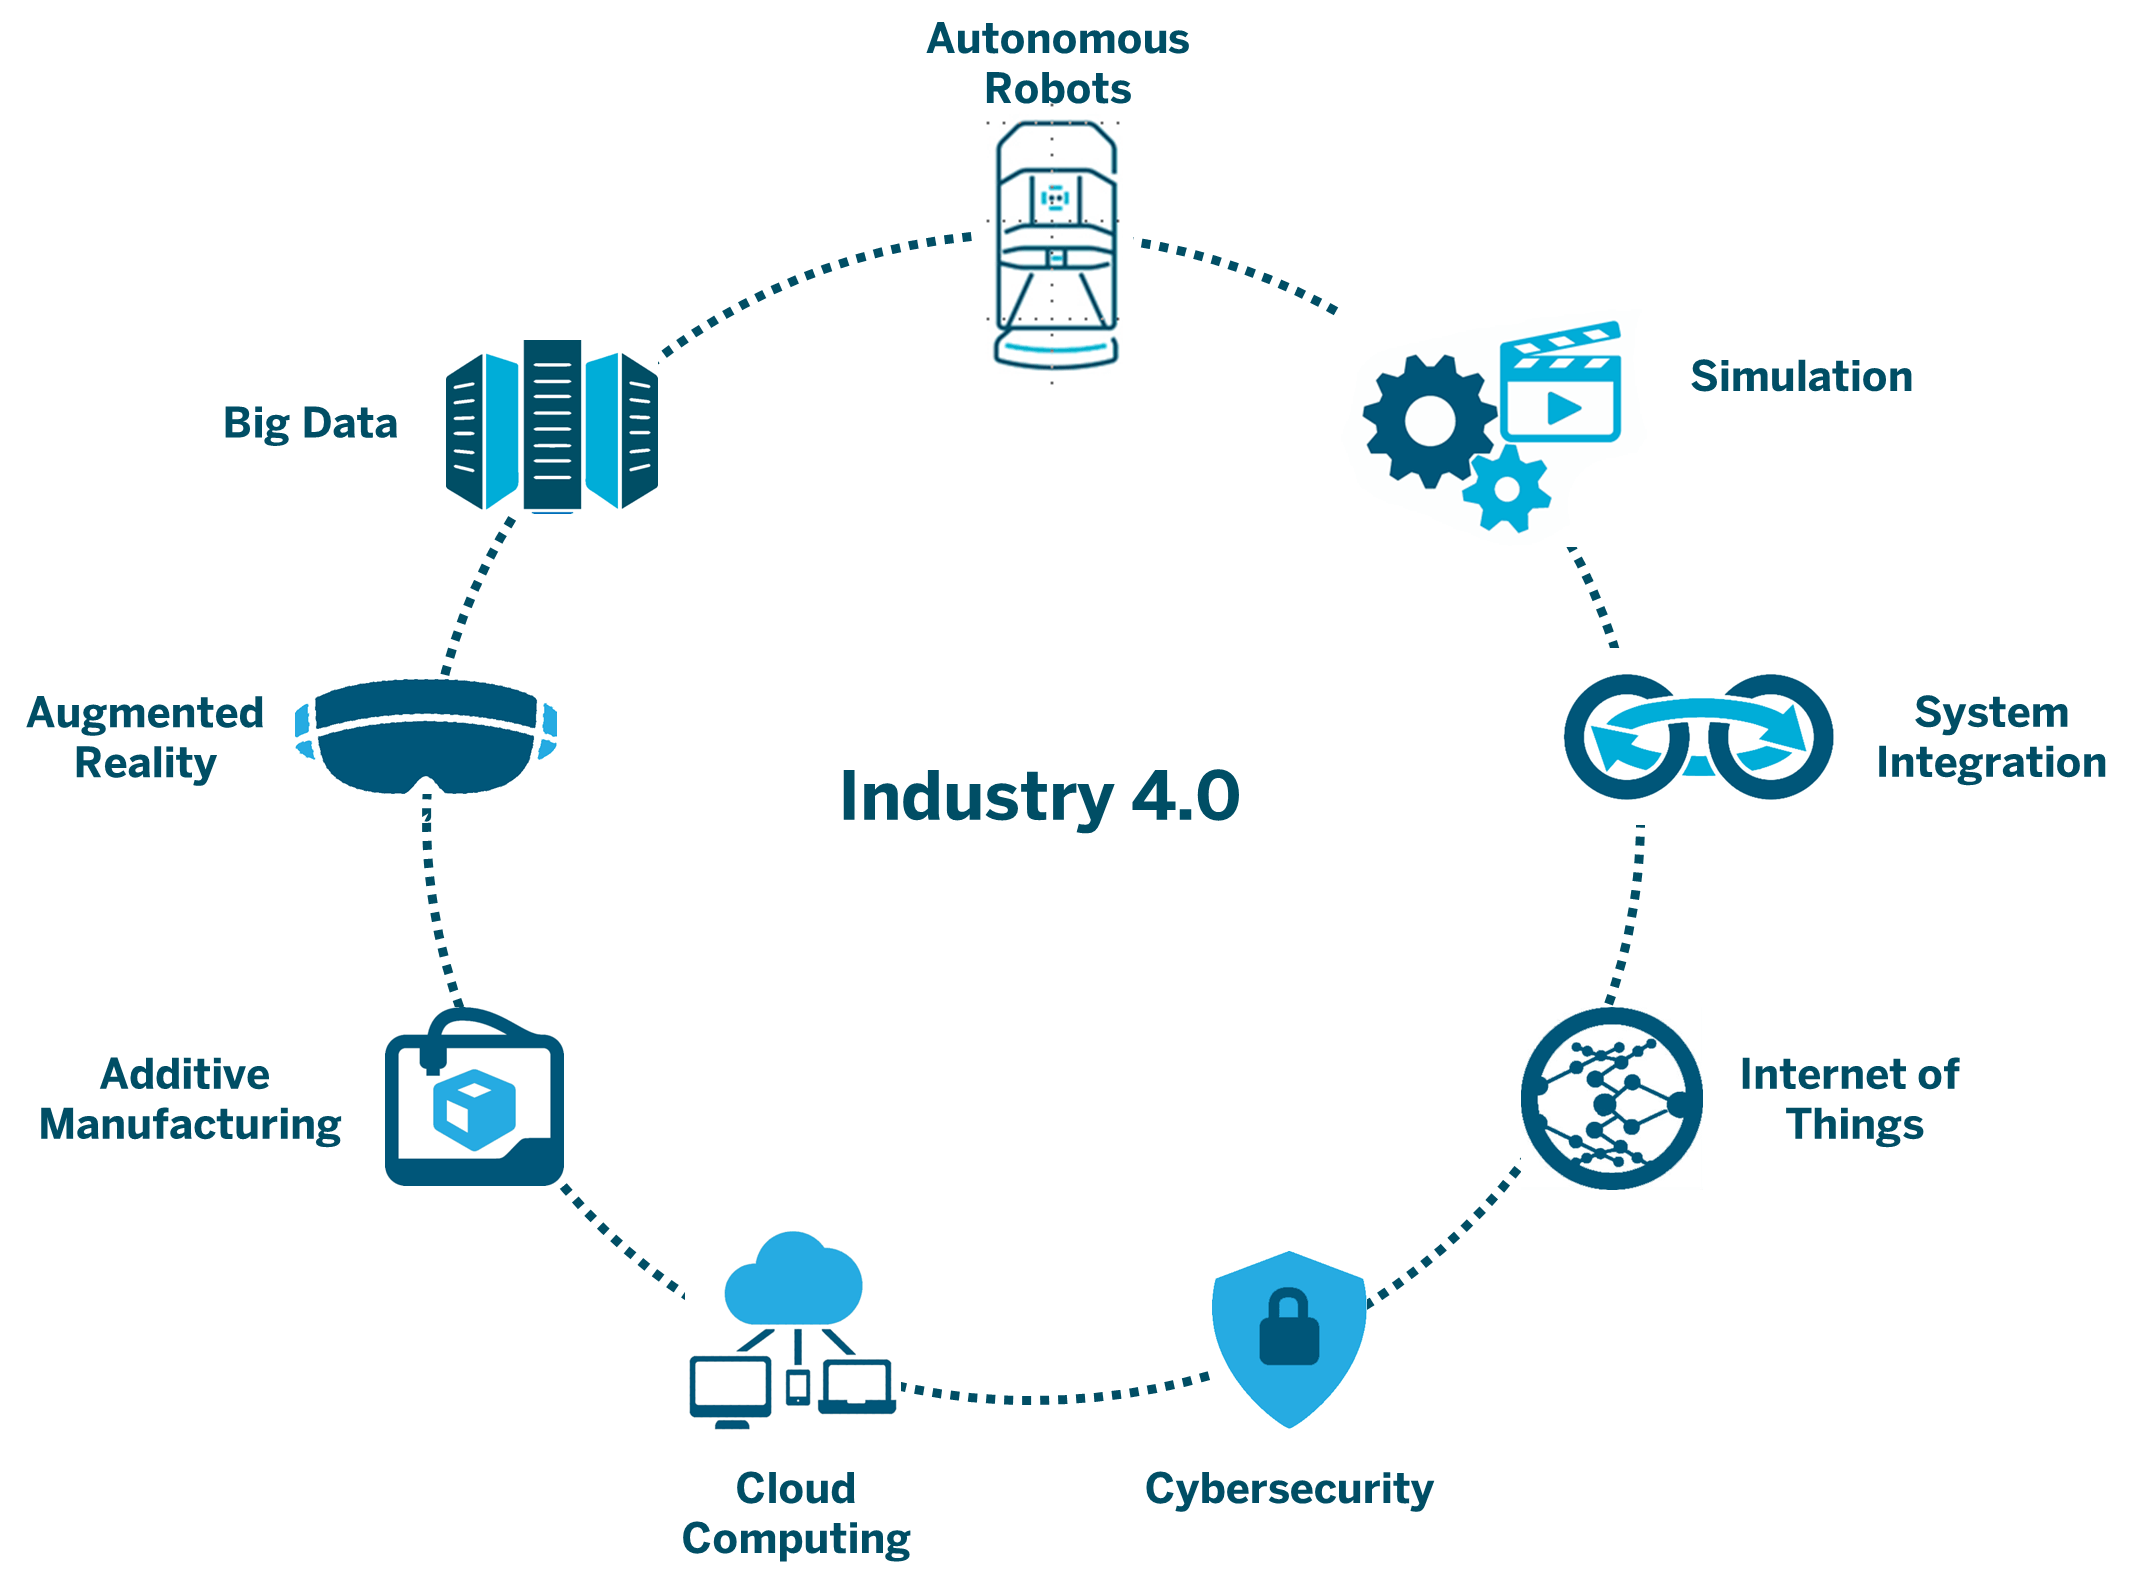
\includegraphics[width=\linewidth]{figures/industry40.png}
	\caption{Ipar 4.0 komponensei \cite{industry40}}
	\label{fig:industry40}
\end{figure}

\subsection{Szállítás}
Nem csak a gyártóiparban lehet elképzelni sok robot irányítását, hanem például szállítás és utazás terén is. A Műegyetemhez legközelebbi metróvonal már évek óta önvezérlőként működik, ugyan egyelőre a hossza befejezetlensége miatt csak tíz körüli metrószerelvény működik egyszerre, azonban ez is egy olyan példája a robotirányításnak, amit minden nap észlelhetünk. Az Amazon házhozszállító cég, amelynek egyébként az AWS (Amazon Web Services) leányvállalata a világ egyik legnagyobb felhőszolgáltatója, már tesztel drónokat, amelyek betöltik a csomagházhozszállítás szerepet. A levegőben való csomagszállítás egyik problémája a \ref{fig:drone-delivery}. ábrán látható.
\begin{figure}
	\centering
	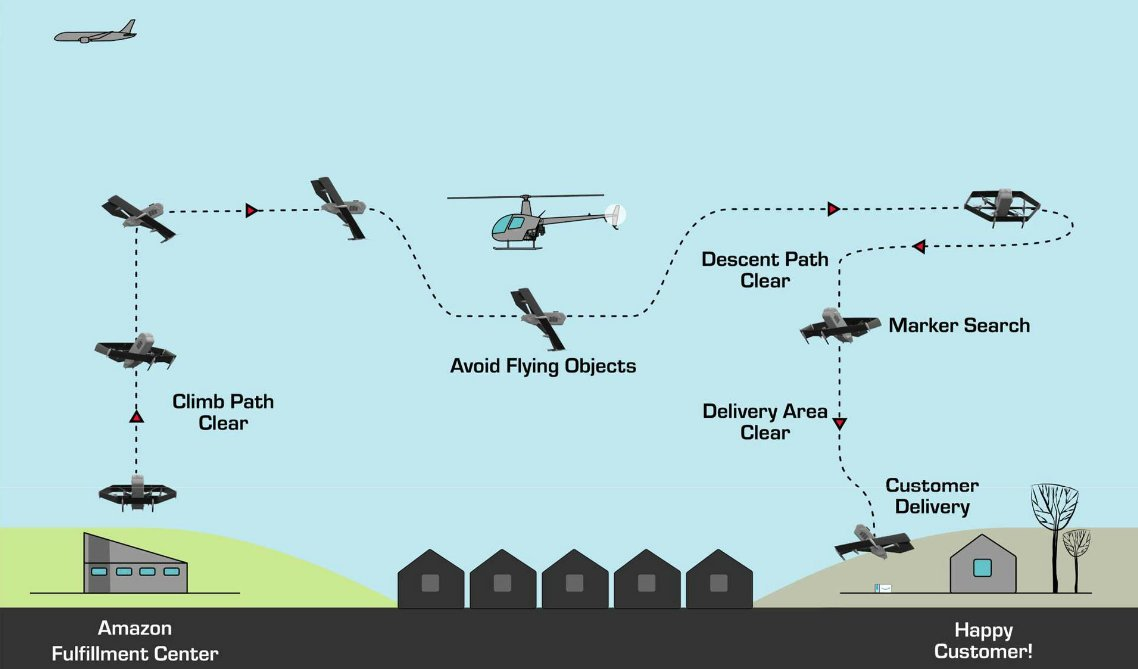
\includegraphics[width=\linewidth]{figures/aws-drone-delivery.jpg}
	\caption{Amazon házhozszállítás problémája drónnal \cite{drone-delivery}}
	\label{fig:drone-delivery}
\end{figure}
\subsection{Mezőgazdaság}
Az agrárvilágban is el lehet képzelni sok robotot kezdve a vetéstől az aratásig, azonban a drónoknak kifejezett szerepe akad a jövőben ebben az iparágban. Használnak ma már automatizált drónokat permetezésre, időszakos állomány megfigyelésre vagy akár kombájn útjának a felderítésére is. Ahogyan a gyártósoroknál, itt is optimalizálhatunk több robot irányítás esetén felhőrendszerrel. A dolgozatban arra keresünk megoldást, hogy ezt milyen eszközrendszerrel érdemes tervezni.
\subsection{Szórakoztatóipar}
Idáig kiderült, hogy rengeteg iparágban alkalmazhatóak a tömegesen irányított robotok, amiket kreativitással könnyű bővíteni. Azonban a szórakoztatóiparban is megjelentek már a tömegesen irányított drónok. Egy jellegzetes példája ennek amerika legnagyobb sporteseménye a Super Bowl 2017-es döntője, ahol 300 drónt használtak fel az égboltra való fényfestéshez a szünetben lévő koncerthez. Ez az esemény egy pillanatfelvétele a \ref{fig:super-bowl}. ábrán látható és az esemény technikai előkészületeiről a \cite{concert} cikkben lehet olvasni.
\begin{figure}
	\centering
	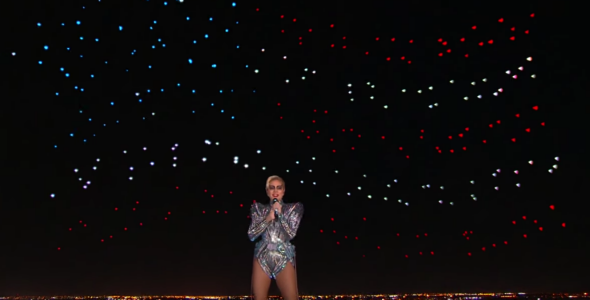
\includegraphics[width=12cm]{figures/super_bowl.png}
	\caption{Lady Gaga 300 drónnal a háttérben a 2017-es Super Bowl döntőjének félideje alatti koncerten \cite{super-bowl-pic}}
	\label{fig:super-bowl}
\end{figure}
Persze ebben a példában egy pár perces feladatról beszélünk az irányított robotok számára, a felhős megoldással pedig egy hosszútávú optimalizációt szeretnénk megadni.

\section{Használt kifejezések}
A hálózati-, virtualizációs- és robotiparban rengeteg rövidítés, mozaikszó és kifejezés létezik, amit főként csak azok ismernek, akik
jelentősebben mélyültek el ezen iparág területén. Két csoportra bontom a diplomatervemhez használt kifejezéseket:
\begin{enumerate}
	\item Azon szakmai kifejezések, amik elterjedtek a mérnöki szakmákban, melyet egy mérnök nem infokommunikációs szakosodás mellett is nagy valószínűséggel ismer és nem kell ismertetnem a tanulmányban. Pár példa a kategóriában, amikre külön nem térek ki, nem oldom fel a szövegben, ilyenek az IPv4, NAT, hálózati réteg, HTTP, CPU, for ciklus.
	\item Azokat a kifejezéseket amik pedig a témához, szakterülethez kapcsolódnak, például a kifejezetten hálózati kommunikáció, virtualizáció, robot, irányítás iparágakba tartozó kifejezések, amiket nem általános mérnöki ismeretek, azokat a szövegben az első használatnál kifejtem, továbbá itt összegyűjtöm.
\end{enumerate}
A tanulmányban használt speciális kifejezések:
\begin{itemize}
	\item QoS (Quality of Service) - A szolgáltatás minőségének a biztosítása
	\item Virtuális gép (Virtual Machine, VM) - Virtualizált önálló teljes értékű operációs rendszer gazdagépen (host-on)
	\item KVM (Kernel-based Virtual Machine) - Kernelhez elosztott időben hozzáférő virtuális gép
	\item Host OS - Hosted virtualizáció esetén a gazdaoperációs rendszer
	\item Guest OS - Hosted virtualizált operációs rendszer a host OS fölött
	\item Hypervisor - A hardveren való virtualizációt megvalósító szoftver
	\item Node - A felhőrendszer egy fizikai eszköze
	\item Cluster/Klaszter - A felhőrendszerbe csatolt fizikai eszközök kapcsolata
	\item Volume - Szolgáltatás/VM háttértára
	\item Vertikális skálázás - Node hozzáadása a cluster-hez
	\item Horizontális skálzás - Node fejlesztés
	\item GCS (Ground Control Station) - Földi irányítóállomás
	\item Földi - Olyan alkalmazás ami nem felhőben fut
	\item Konténer Registry - Konténereket tároló és menedzselő rendszer
\end{itemize}


% Acknowledgements
%~~~~~~~~~~~~~~~~~~~~~~~~~~~~~~~~~~~~~~~~~~~~~~~~~~~~~~~~~~~~~~~~~~~~~~~~~~~~~~~~~~~~~~
%%----------------------------------------------------------------------------
\chapter*{\koszonetnyilvanitas}\addcontentsline{toc}{chapter}{\koszonetnyilvanitas}
%----------------------------------------------------------------------------

Ez nem kötelező, akár törölhető is. Ha a szerző szükségét érzi, itt lehet köszönetet nyilvánítani azoknak, akik hozzájárultak munkájukkal ahhoz, hogy a hallgató a szakdolgozatban vagy diplomamunkában leírt feladatokat sikeresen elvégezze. A konzulensnek való köszönetnyilvánítás sem kötelező, a konzulensnek hivatalosan is dolga, hogy a hallgatót konzultálja.


% List of Figures, Tables
%~~~~~~~~~~~~~~~~~~~~~~~~~~~~~~~~~~~~~~~~~~~~~~~~~~~~~~~~~~~~~~~~~~~~~~~~~~~~~~~~~~~~~~
%\listoffigures\addcontentsline{toc}{chapter}{\listfigurename}
%\listoftables\addcontentsline{toc}{chapter}{\listtablename}


% Bibliography
%~~~~~~~~~~~~~~~~~~~~~~~~~~~~~~~~~~~~~~~~~~~~~~~~~~~~~~~~~~~~~~~~~~~~~~~~~~~~~~~~~~~~~~
%\addcontentsline{toc}{chapter}{\bibname}
%\bibliography{bib/mybib}


% Appendix
%~~~~~~~~~~~~~~~~~~~~~~~~~~~~~~~~~~~~~~~~~~~~~~~~~~~~~~~~~~~~~~~~~~~~~~~~~~~~~~~~~~~~~~
%%----------------------------------------------------------------------------
\appendix
%----------------------------------------------------------------------------
\chapter*{\fuggelek}\addcontentsline{toc}{chapter}{\fuggelek}
\setcounter{chapter}{\appendixnumber}
%\setcounter{equation}{0} % a fofejezet-szamlalo az angol ABC 6. betuje (F) lesz
\numberwithin{equation}{section}
\numberwithin{figure}{section}
\numberwithin{lstlisting}{section}
%\numberwithin{tabular}{section}

%----------------------------------------------------------------------------
\section{A TeXstudio felülete}
%----------------------------------------------------------------------------
\begin{figure}[!ht]
\centering
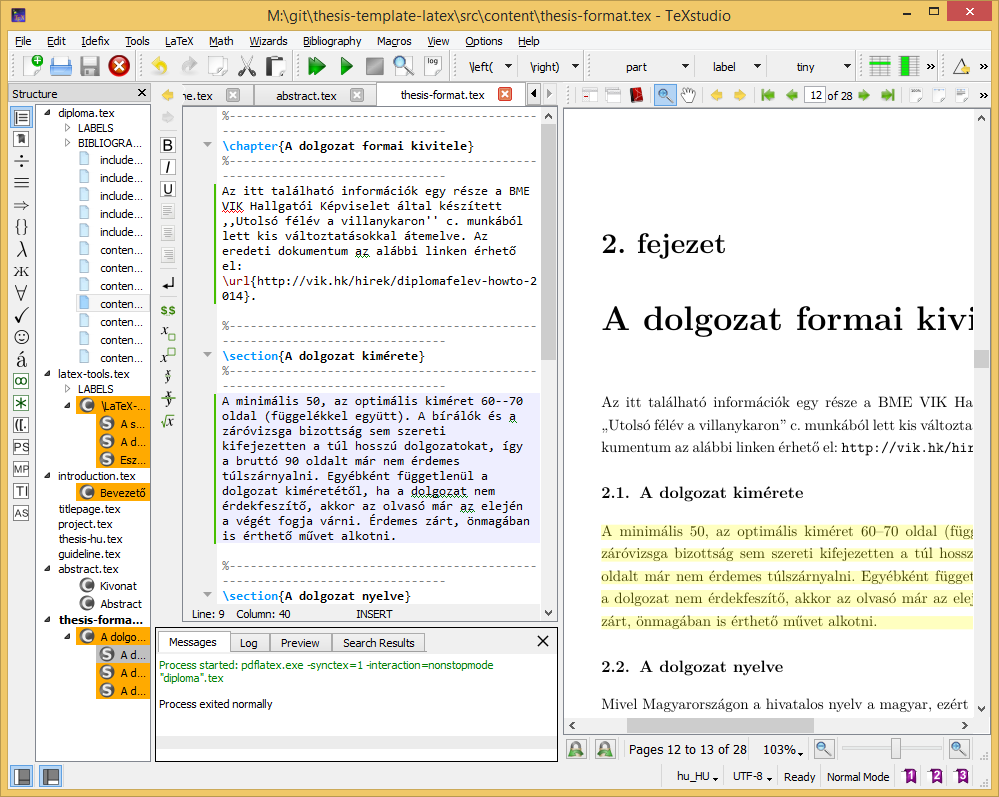
\includegraphics[width=150mm, keepaspectratio]{figures/TeXstudio.png}
\caption{A TeXstudio \LaTeX-szerkesztő.} 
\end{figure}

%----------------------------------------------------------------------------
\clearpage\section{Válasz az ,,Élet, a világmindenség, meg minden'' kérdésére}
%----------------------------------------------------------------------------
A Pitagorasz-tételből levezetve
\begin{align}
c^2=a^2+b^2=42.
\end{align}
A Faraday-indukciós törvényből levezetve
\begin{align}
\rot E=-\frac{dB}{dt}\hspace{1cm}\longrightarrow \hspace{1cm}
U_i=\oint\limits_\mathbf{L}{\mathbf{E}\mathbf{dl}}=-\frac{d}{dt}\int\limits_A{\mathbf{B}\mathbf{da}}=42.
\end{align}


%\label{page:last}
\end{document}
